%\section{Learning with/of Neural Path Features}
\textbf{Optimisation:} The ability of DNNs to fit data has been demonstrated in the past \cite{ben}, i.e., they can fit even random labels, and random pixels of standard datasets such as MNIST. However, for standard DNNs with ReLU gates, with no bias parameters, a dataset with $n=2$ points namely $(x,1)$ and $(2x,-1)$ for some $x\in \R^{d_{in}}$ cannot be memorised. The reason is that the gating values are the same for both $x$ and $2x$ (for that matter any positive scaling of $x$), and hence $\phi_{2x,\G_t }= 2\phi_{x,\G_t }$, and thus it not possible to fit arbitrary values for $\hat{y}_t(x)$ and $\hat{y}_t(2x)$.\\
\textbf{Generalisation:} We trained DGN on standard datasets namely MNIST and CIFAR-10, under the following conditions: i) the gates are frozen $\G_t=\G_0,\forall t\geq 0$ and ii) the gating values are obtained from a ReLU network, which acts as the gating network (see \Cref{tb:dgn}). Since, the gates are frozen, the NPFs are fixed and the SGD learns only the path values. We compare the performance of $4$ different NPFs, wherein, the gates are copied from i) from a randomly initialised ReLU network (untrained), ii) from a ReLU network trained with good dataset iii) ReLU network trained on random labels and iv) ReLU network trained on random pixels.
\FloatBarrier
\begin{table}[h]
\begin{tabular}{|c|c|c|c|c|c|c|}\hline
&&&&\multicolumn{3}{c|}{NPF (trained)}\\\cline{5-7}
$(w,d)$	&Dataset		&ReLU		&NPF(untrained) 		&Good 		&Random Labels 	&Random Pixel\\\hline
$(128,6)$	& MNIST 		& $98.15$ 		&$96$ 		&$98.3$		&$92.6$			&$94.3$\\\hline
$(256,6)$	& MNIST 		& $98.5$ 		&$96.6$ 		&$98.4$		&$92.0$			&$81.1$\\\hline
\end{tabular}
\caption{Shows the training and generalisation performance of various GaLU network. Here, non-learned stands for gates from a randomly initialised ReLU network.}
\label{tb:npfs}
\end{table}
\FloatBarrier
\begin{wrapfigure}{h}{0.3\textwidth}
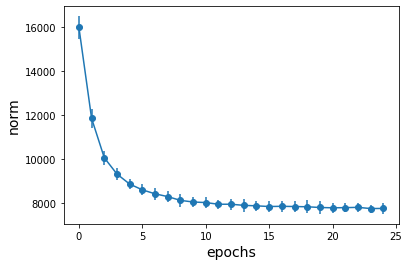
\includegraphics[scale=0.25]{figs/path-gram.png}
\caption{\label{fig:frog1}This is a figure caption.}
\end{wrapfigure}
\textbf{Feature Learning:} We consider ``Binary''-MNIST data set with two classes namely digits $4$ and $7$, with the labels taking values in $\{-1,+1\}$ and squared loss. We trained a standard DNN with ReLU activation ($w=100$, $d=5$). Recall that $H_t=\Phi^\top_t\Phi_t$  (the Gram matrix of the features) and let $\widehat{H}_t=\frac{1}{trace(H_t)}H_t$ be its normalised counterpart. For a subset size, $n'=200$ ($100$ examples per class) we plot $\nu_t=y^\top (\widehat{H}_t)^{-1} y$, (where $y\in\{-1,1\}^{200}$ is the labeling function), and observe that $\nu_t$ reduces as training proceeds (see first plot in \Cref{fig:gen}). Note that $\nu_t=\sum_{i=1}^{n'}(u_{i,t}^\top y)^2 (\hat{\rho}_{i,t})^{-1}$, where $u_{i,t}\in \R^{n'}$ are the orthonormal eigenvectors of $\widehat{H}_t$ and $\hat{\rho}_{i,t},i\in[n']$ are the corresponding eigenvalues. Since $\sum_{i=1}^{n'}\hat{\rho}_{i,t}=1$, the only way $\nu_t$ reduces is when more and more energy gets concentrated on $\hat{\rho}_{i,t}$s for which $(u_{i,t}^\top y)^2$s are also high. However, in $H_t=(x^\top x)\odot \lambda_t$, only $\lambda_t$ changes with time. Thus, $\lambda_t(s,s')$ which is a measure of overlap of sub-networks active for input examples $s,s'\in[n]$, changes in a manner to reduce $\nu_t$. We can thus infer that the \emph{right} active sub-networks are learned over the course of training. We now summarise the insights obtained from these experiments in the following remarks:\hfill\\
